\documentclass{standalone}
\usepackage{tikz}
\usetikzlibrary{patterns, positioning}


\begin{document}
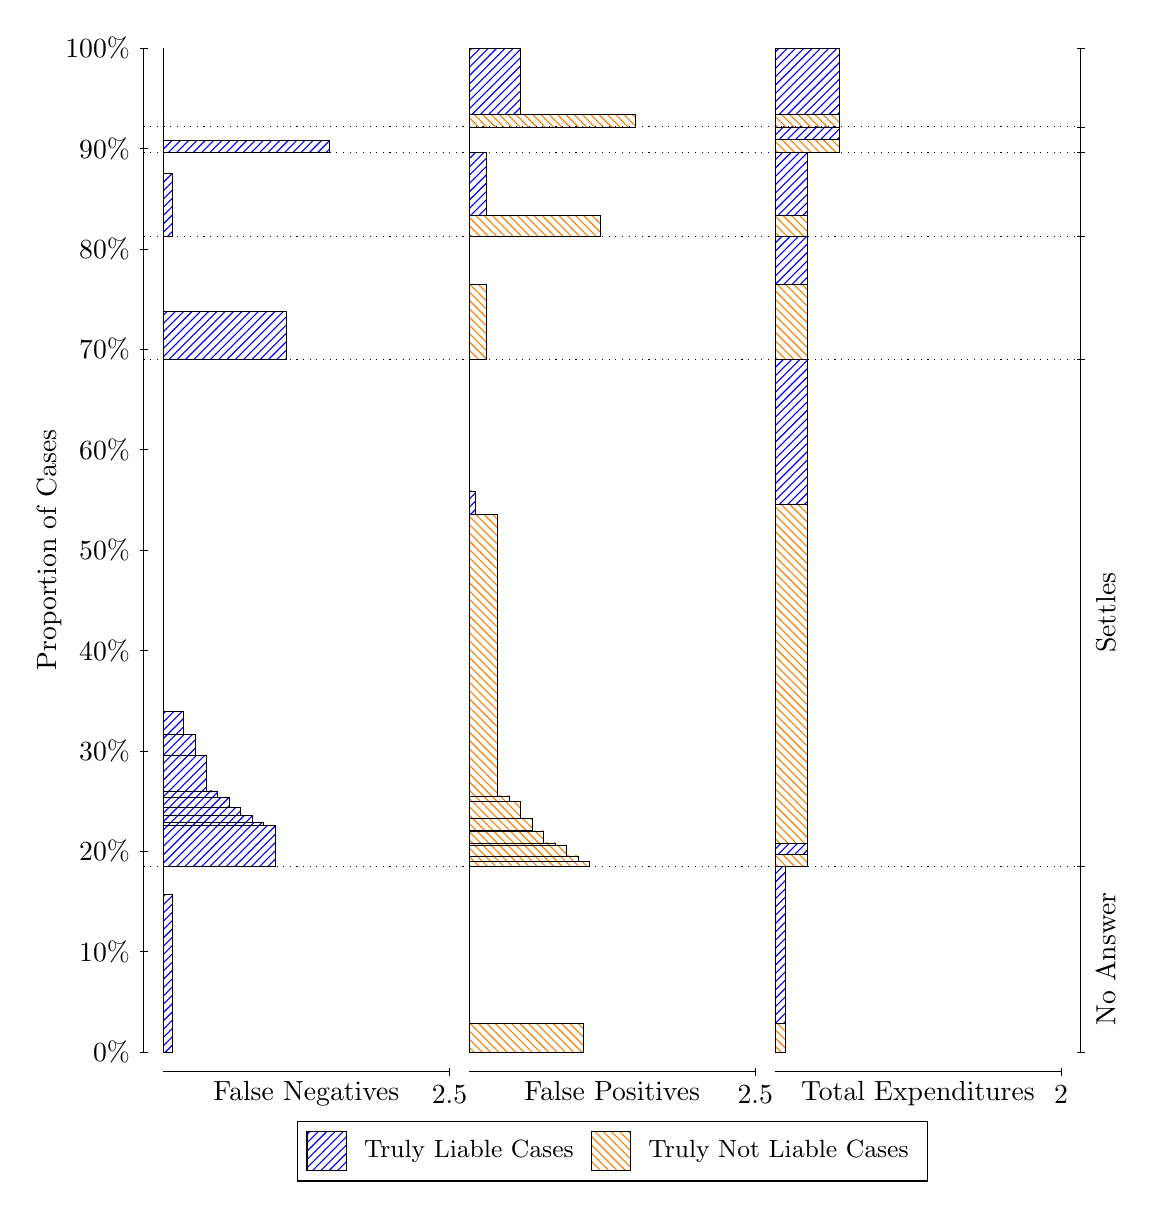
\begin{tikzpicture}
\draw[black, very thin] (1.5,1.75) -- (1.5,14.5);
\node[rotate=90, text=black, anchor=center] at (0.3, 8.125) {Proportion of Cases};
\draw[black, very thin] (1.45,1.75) -- (1.55,1.75);
\node[text=black, anchor=east] at (1.45, 1.75) {0\%};
\draw[black, very thin] (1.45,3.025) -- (1.55,3.025);
\node[text=black, anchor=east] at (1.45, 3.025) {10\%};
\draw[black, very thin] (1.45,4.3) -- (1.55,4.3);
\node[text=black, anchor=east] at (1.45, 4.3) {20\%};
\draw[black, very thin] (1.45,5.575) -- (1.55,5.575);
\node[text=black, anchor=east] at (1.45, 5.575) {30\%};
\draw[black, very thin] (1.45,6.85) -- (1.55,6.85);
\node[text=black, anchor=east] at (1.45, 6.85) {40\%};
\draw[black, very thin] (1.45,8.125) -- (1.55,8.125);
\node[text=black, anchor=east] at (1.45, 8.125) {50\%};
\draw[black, very thin] (1.45,9.4) -- (1.55,9.4);
\node[text=black, anchor=east] at (1.45, 9.4) {60\%};
\draw[black, very thin] (1.45,10.675) -- (1.55,10.675);
\node[text=black, anchor=east] at (1.45, 10.675) {70\%};
\draw[black, very thin] (1.45,11.95) -- (1.55,11.95);
\node[text=black, anchor=east] at (1.45, 11.95) {80\%};
\draw[black, very thin] (1.45,13.225) -- (1.55,13.225);
\node[text=black, anchor=east] at (1.45, 13.225) {90\%};
\draw[black, very thin] (1.45,14.5) -- (1.55,14.5);
\node[text=black, anchor=east] at (1.45, 14.5) {100\%};

\draw[black, very thin] (13.4,1.75) -- (13.4,14.5);
\draw[black, very thin] (13.35,1.75) -- (13.45,1.75);
\node[anchor=west] at (13.35, 1.75) {};
\draw[black, very thin] (13.35,4.1093) -- (13.45,4.1093);
\node[anchor=west] at (13.35, 4.1093) {};
\draw[black, very thin] (13.35,10.545) -- (13.45,10.545);
\node[anchor=west] at (13.35, 10.545) {};
\draw[black, very thin] (13.35,12.106) -- (13.45,12.106);
\node[anchor=west] at (13.35, 12.106) {};
\draw[black, very thin] (13.35,13.176) -- (13.45,13.176);
\node[anchor=west] at (13.35, 13.176) {};
\draw[black, very thin] (13.35,13.499) -- (13.45,13.499);
\node[anchor=west] at (13.35, 13.499) {};
\draw[black, very thin] (13.35,14.5) -- (13.45,14.5);
\node[anchor=west] at (13.35, 14.5) {};

\draw[black, very thin, pattern color=blue, pattern=north east lines] (1.75,1.75) rectangle (1.859,3.7477);
\draw[black, very thin, pattern color=orange, pattern=north west lines] (1.75,3.7477) rectangle (1.75,4.1093);
\draw[black, very thin, pattern color=blue, pattern=north east lines] (1.75,4.1093) rectangle (3.167,4.6253);
\draw[black, very thin, pattern color=blue, pattern=north east lines] (1.75,4.6253) rectangle (3.0217,4.664);
\draw[black, very thin, pattern color=blue, pattern=north east lines] (1.75,4.664) rectangle (2.8763,4.7544);
\draw[black, very thin, pattern color=blue, pattern=north east lines] (1.75,4.7544) rectangle (2.731,4.8589);
\draw[black, very thin, pattern color=blue, pattern=north east lines] (1.75,4.8589) rectangle (2.5857,4.987);
\draw[black, very thin, pattern color=blue, pattern=north east lines] (1.75,4.987) rectangle (2.4403,5.0658);
\draw[black, very thin, pattern color=blue, pattern=north east lines] (1.75,5.0658) rectangle (2.295,5.5141);
\draw[black, very thin, pattern color=blue, pattern=north east lines] (1.75,5.5141) rectangle (2.1497,5.7795);
\draw[black, very thin, pattern color=blue, pattern=north east lines] (1.75,5.7795) rectangle (2.0043,6.0782);
\draw[black, very thin, pattern color=orange, pattern=north west lines] (1.75,6.0782) rectangle (1.75,10.545);
\draw[black, very thin, pattern color=blue, pattern=north east lines] (1.75,10.545) rectangle (3.3123,11.157);
\draw[black, very thin, pattern color=orange, pattern=north west lines] (1.75,11.157) rectangle (1.75,12.106);
\draw[black, very thin, pattern color=blue, pattern=north east lines] (1.75,12.106) rectangle (1.859,12.905);
\draw[black, very thin, pattern color=orange, pattern=north west lines] (1.75,12.905) rectangle (1.75,13.176);
\draw[black, very thin, pattern color=blue, pattern=north east lines] (1.75,13.176) rectangle (3.8573,13.33);
\draw[black, very thin, pattern color=orange, pattern=north west lines] (1.75,13.33) rectangle (1.75,13.499);
\draw[black, very thin, pattern color=orange, pattern=north west lines] (1.75,13.499) rectangle (1.75,13.657);
\draw[black, very thin, pattern color=blue, pattern=north east lines] (1.75,13.657) rectangle (1.75,14.5);
\draw[black, very thin, pattern color=orange, pattern=north west lines] (5.6333,1.75) rectangle (7.0867,2.1115);
\draw[black, very thin, pattern color=blue, pattern=north east lines] (5.6333,2.1115) rectangle (5.6333,4.1093);
\draw[black, very thin, pattern color=orange, pattern=north west lines] (5.6333,4.1093) rectangle (7.1593,4.1664);
\draw[black, very thin, pattern color=orange, pattern=north west lines] (5.6333,4.1664) rectangle (7.014,4.2397);
\draw[black, very thin, pattern color=orange, pattern=north west lines] (5.6333,4.2397) rectangle (6.8687,4.3693);
\draw[black, very thin, pattern color=orange, pattern=north west lines] (5.6333,4.3693) rectangle (6.7233,4.4064);
\draw[black, very thin, pattern color=orange, pattern=north west lines] (5.6333,4.4064) rectangle (6.578,4.5579);
\draw[black, very thin, pattern color=orange, pattern=north west lines] (5.6333,4.5579) rectangle (6.4327,4.5596);
\draw[black, very thin, pattern color=orange, pattern=north west lines] (5.6333,4.5596) rectangle (6.4327,4.7214);
\draw[black, very thin, pattern color=orange, pattern=north west lines] (5.6333,4.7214) rectangle (6.2873,4.9282);
\draw[black, very thin, pattern color=orange, pattern=north west lines] (5.6333,4.9282) rectangle (6.142,5.0015);
\draw[black, very thin, pattern color=orange, pattern=north west lines] (5.6333,5.0015) rectangle (5.9967,8.5762);
\draw[black, very thin, pattern color=blue, pattern=north east lines] (5.6333,8.5762) rectangle (5.706,8.8749);
\draw[black, very thin, pattern color=blue, pattern=north east lines] (5.6333,8.8749) rectangle (5.6333,10.545);
\draw[black, very thin, pattern color=orange, pattern=north west lines] (5.6333,10.545) rectangle (5.8513,11.495);
\draw[black, very thin, pattern color=blue, pattern=north east lines] (5.6333,11.495) rectangle (5.6333,12.106);
\draw[black, very thin, pattern color=orange, pattern=north west lines] (5.6333,12.106) rectangle (7.3047,12.377);
\draw[black, very thin, pattern color=blue, pattern=north east lines] (5.6333,12.377) rectangle (5.8513,13.176);
\draw[black, very thin, pattern color=orange, pattern=north west lines] (5.6333,13.176) rectangle (5.6333,13.344);
\draw[black, very thin, pattern color=blue, pattern=north east lines] (5.6333,13.344) rectangle (5.6333,13.499);
\draw[black, very thin, pattern color=orange, pattern=north west lines] (5.6333,13.499) rectangle (7.7407,13.657);
\draw[black, very thin, pattern color=blue, pattern=north east lines] (5.6333,13.657) rectangle (6.2873,14.5);
\draw[black, very thin, pattern color=orange, pattern=north west lines] (9.5167,1.75) rectangle (9.6529,2.1115);
\draw[black, very thin, pattern color=blue, pattern=north east lines] (9.5167,2.1115) rectangle (9.6529,4.1093);
\draw[black, very thin, pattern color=orange, pattern=north west lines] (9.5167,4.1093) rectangle (9.9254,4.2625);
\draw[black, very thin, pattern color=blue, pattern=north east lines] (9.5167,4.2625) rectangle (9.9254,4.3961);
\draw[black, very thin, pattern color=orange, pattern=north west lines] (9.5167,4.3961) rectangle (9.9254,8.7098);
\draw[black, very thin, pattern color=blue, pattern=north east lines] (9.5167,8.7098) rectangle (9.9254,10.545);
\draw[black, very thin, pattern color=orange, pattern=north west lines] (9.5167,10.545) rectangle (9.9254,11.495);
\draw[black, very thin, pattern color=blue, pattern=north east lines] (9.5167,11.495) rectangle (9.9254,12.106);
\draw[black, very thin, pattern color=orange, pattern=north west lines] (9.5167,12.106) rectangle (9.9254,12.377);
\draw[black, very thin, pattern color=blue, pattern=north east lines] (9.5167,12.377) rectangle (9.9254,13.176);
\draw[black, very thin, pattern color=orange, pattern=north west lines] (9.5167,13.176) rectangle (10.334,13.344);
\draw[black, very thin, pattern color=blue, pattern=north east lines] (9.5167,13.344) rectangle (10.334,13.499);
\draw[black, very thin, pattern color=orange, pattern=north west lines] (9.5167,13.499) rectangle (10.334,13.657);
\draw[black, very thin, pattern color=blue, pattern=north east lines] (9.5167,13.657) rectangle (10.334,14.5);
\draw[black, dotted] (1.5,4.1093) -- (13.4,4.1093);
\draw[black, dotted] (1.5,10.545) -- (13.4,10.545);
\draw[black, dotted] (1.5,12.106) -- (13.4,12.106);
\draw[black, dotted] (1.5,13.176) -- (13.4,13.176);
\draw[black, dotted] (1.5,13.499) -- (13.4,13.499);
\draw[black, very thin] (1.75,1.5) -- (5.3833,1.5);
\node[text=black, anchor=north] at (3.5667, 1.5) {False Negatives};
\draw[black, very thin] (5.3833,1.45) -- (5.3833,1.55);
\node[text=black, anchor=north] at (5.3833, 1.45) {2.5};

\draw[black, very thin] (5.6333,1.5) -- (9.2667,1.5);
\node[text=black, anchor=north] at (7.45, 1.5) {False Positives};
\draw[black, very thin] (9.2667,1.45) -- (9.2667,1.55);
\node[text=black, anchor=north] at (9.2667, 1.45) {2.5};

\draw[black, very thin] (9.5167,1.5) -- (13.15,1.5);
\node[text=black, anchor=north] at (11.333, 1.5) {Total Expenditures};
\draw[black, very thin] (13.15,1.45) -- (13.15,1.55);
\node[text=black, anchor=north] at (13.15, 1.45) {2};

\node[text=black, centered, rotate=90] at (13.72, 2.9296) {No Answer};
\node[text=black, centered, rotate=90] at (13.72, 7.3272) {Settles};





\draw (7.449999999999999,1.5) node[draw=none] (baseCoordinate) {};
\begin{scope}[align=center]
        \matrix[scale=0.5, draw=black, below=0.5cm of baseCoordinate, nodes={draw}, column sep=0.1cm]{
            \node[rectangle, draw, minimum width=0.5cm, minimum height=0.5cm, pattern color=blue, pattern=north east lines] {}; &
            \node[draw=none, font=\small, text=black] (B) {Truly Liable Cases}; &
            \node[rectangle, draw, minimum width=0.5cm, minimum height=0.5cm, pattern color=orange, pattern=north west lines] {}; &
            \node[draw=none, font=\small, text=black] (B) {Truly Not Liable Cases}; \\
            };
\end{scope}

\end{tikzpicture}
\end{document}